\chapter{\textbf{Технологический раздел}}

В данном разделе описываются средства реализации, их преимущества, схема разработанного программного обеспечения, приводятся листинги исходного кода и изображения интерфейса пользователя.

\section{Входные и выходные данные}

Входными данными является фотография документа, удостоверяющего личность. Документ на фотографии должен быть хорошо освещен, находиться в фокусе, не смазан и занимать не менее 70\% площади фотографии, поворот документ вокруг любой оси должен быть менее 15 градусов.

Выходные данные -- название класса документа, к которому он относится.

\section{Язык программирования}

В качестве языка реализации разрабатываемого метода был выбран Python версии 3.7 \cite{python}. Использование данного языка в области машинного обучения и нейронных сетей крайне популярно, что благоприятно сказывается на доступности документации и библиотек в данной предметной области.

\subsection{Библиотеки}

В разработанном ПО были использованы следующие библиотеки.

\begin{enumerate}
\item[1.] NLTK (Natural Language Toolkit) \cite{nltk} -- пакет библиотек и программ для символьной и статистической обработки естественного языка, написанных на языке программирования Python. Была использована для предобработки текста.

\item[2.] Scikit-learn \cite{scikit} является библиотекой для работы с машинным обучением. Была использована при реализации метода опорных векторов и при обучении ее и также googlenet.

\item[3.] PyTesseract \cite{pytesseract} -- это пакет Python для OCR, соотвественно был использован для извлечения текста с изображений.

\item[4.] OpenCV \cite{opencv} представляет собой самую популярную библиотеку для работы с компьютерным зрением, обработки изображений и набором сопутствующих алгоритмов.

В данной работе были использованы базовые структуры (матрицы изображений, вектора), а также модули загрузки изображений с диска.

\item[5.] TensorFlow \cite{tensorflow} -- это библиотека с открытым исходным кодом, предназначенная для машинного обучения. С помощью данной библиотеки, а точнее ее надстройкой Keras \cite{keras}, была написана модель googlenet.

\item[6.] PyQt \cite{pyqt} -- кроссплатформенный фреймворк для разработки ПО на языках C++, Python, Ruby и других. Qt был использован для создания интерфейса разработанного программного обеспечения. 
\end{enumerate}

\section{UML диаграмма разработанного ПО }

ПО было поделено на следующие основные модули.
\begin{itemize}
\item Классификатор по визуальным признакам.
\item Классификатор по текстовым признакам.
\item Модуль предобработки.
\item Интерфейс.
\end{itemize}

Полная UML диаграмма разработанного ПО представлена на рисунке \ref{img:uml}.

\begin{figure}[H]
	\centering
	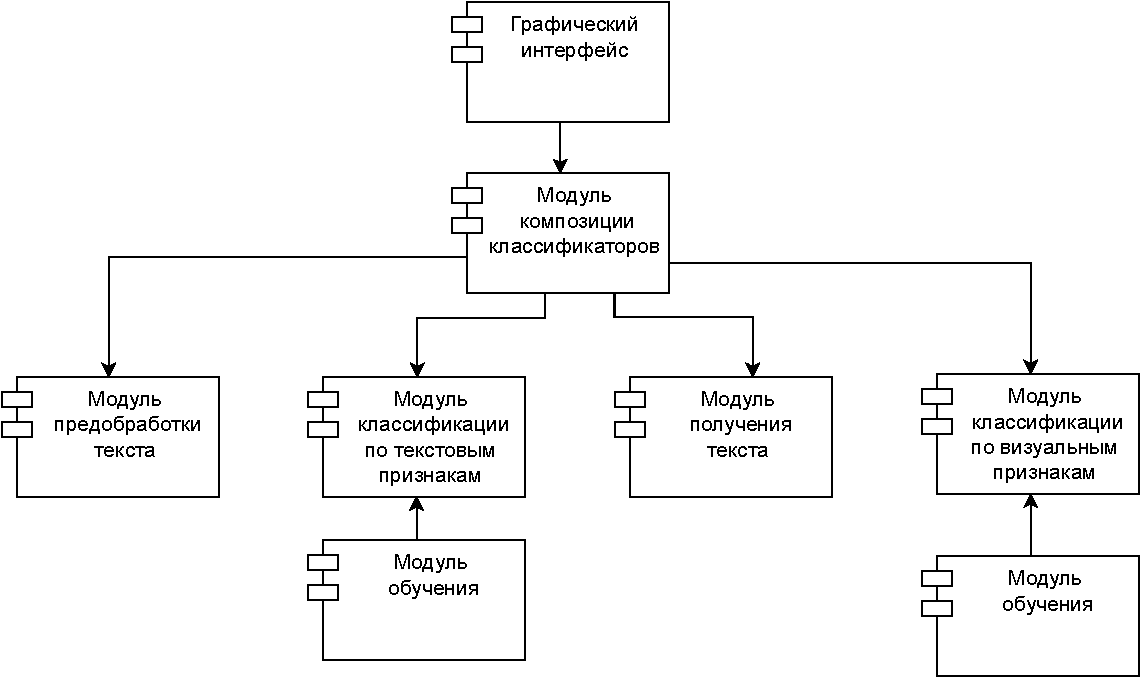
\includegraphics[scale=1]{uml}
	\caption{UML диаграмма разработанного ПО. }
	\label{img:uml}
\end{figure}

Как было сказано выше для классификации документа по визуальным признакам была реализована модель googlenet, её программную реализацию можно посмотреть в листинге \ref{lst:googlenet}. Нейронная сеть обучалась на описанной выше выборке.

После извлечения текста с изображения необходимо его предобработать перед классификацией, программная реализация алгоритма представлена в листинге \ref{lst:text}. 

STOPWORDS -- семантически незначимые слова, в данном случае необходимо рассмотреть слова из 6 языков, так как рассматриваются документы 6 стран.

Далее останется объединить классификаторы в ансамбль, код реализации представлен в листинге \ref{lst:concat}. 

\section{Пользовательский интерфейс }

Пример работы программы для двух типов документов -- визы Германии и водительского удостоверения нового образца, представлен на рисунках \ref{img:vu}, \ref{img:visa}.

\begin{figure}[H]
	\centering
	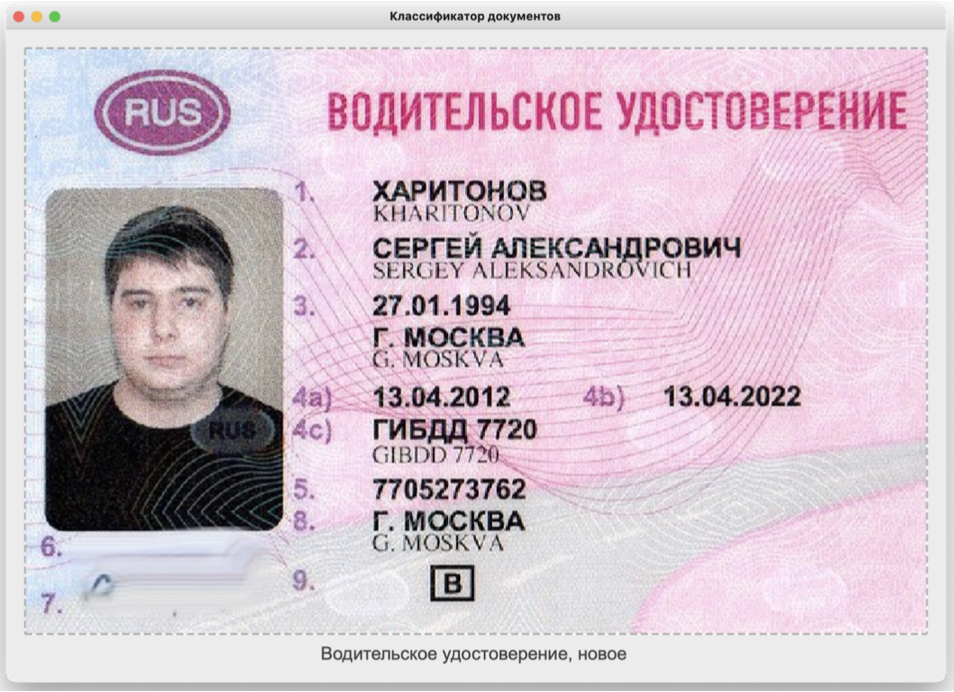
\includegraphics[scale=0.5]{vu}
	\caption{Пример работы программы для типа документа -- Водительское удостоверение нового образца. }
	\label{img:vu}
\end{figure}

\begin{figure}[H]
	\centering
	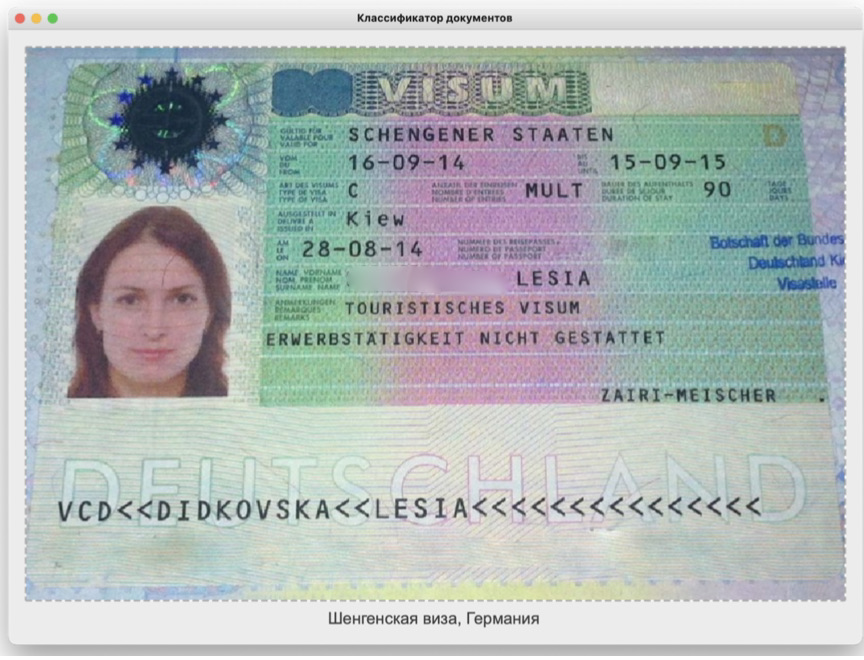
\includegraphics[scale=0.5]{visa}
	\caption{Пример работы программы для типа документа -- Виза. }
	\label{img:visa}
\end{figure}

\section{Вывод}

В разделе проведены выбор средств реализации (язык программирования Python), а также используемых библиотеки (NLTK, Scikit-learn, PyTesseract, OpenCV, TensorFlow, PyQt), предоставлены данные о том, где использовались эти библиотеки. Был разработан метод, описан и разработан пользовательский интерфейс для просмотра результатов, модели классификаторов обучены. Также, были описаны входные (фотография с документом) и выходные (класс документа) данные.
